\scanpage{40}\mspage{39}
% @axiom
\uline{Cont} 5 Soient $X.Y\in M$, $X$ et $Y$ \uline{disjoints}. Alors pour $X'\ll X$ et $Y'\ll Y$, $X'$ et $Y'$ sont \deleted{disjoints} \deleted{compatibles} disjoints
\margin{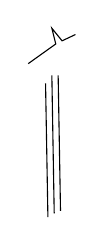
\begin{tikzpicture}[x=1cm,y=1cm]\draw (0,0)--(-.03,1.7) (.08,.05)--(.05,1.8) (.16,.08)--(.13,1.8);\draw (-.25,1.95)--(.1,2.2)--(.05,2.4)--(.18,2.24)--(.35,2.32);\end{tikzpicture}}
% @sim
% slanted
\margin{S'apparente à \uline{Cont} 2 (page 33)}
% @cancelone

\figure{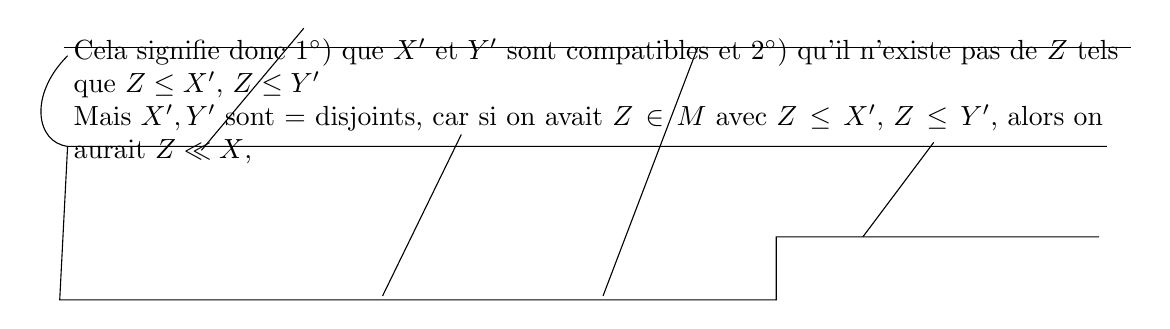
\begin{tikzpicture}[x=1cm,y=1cm]
\node[anchor=north west,inner sep=2pt,text width=13.5cm] (cancelled) at (0,0) {\deleted{Cela signifie donc $1^\circ$) que $X'$ et $Y'$ sont compatibles et $2^\circ$) qu'il n'existe pas de $Z$ tels que $Z\leq X'$, $Z\leq Y'$}
% @canceltwo

\deleted{Mais $X',Y'$ sont $=$ disjoints, car si on avait \inserted{$Z\in M$ avec} $Z\leq X'$, $Z\leq Y'$, alors on aurait $Z\ll X$,}};
\draw (-.05,-.2)--(13.5,-.2);
\draw (0,-.3) .. controls (-.5,-.8) and (-.4,-1.4) .. (0,-1.45)--(13.2,-1.45);
\draw (0,-1.45)--(-.1,-3.4)--(9,-3.4)--(9,-2.6)--(13.1,-2.6);
\draw (3,.05)--(1.7,-1.5) (5,-1.3)--(4,-3.35) (8,-.2)--(6.8,-3.35) (11,-1.4)--(10.1,-2.6);
\end{tikzpicture}}
% @split

Se décompose en deux

% @splita
\textcircled{\scriptsize a} Sous les condition de Cont 5, $X'$ et $Y'$ st \uline{compatibles}
% @noz

\textcircled{\scriptsize b} \deleted{Si $Z$} $\nexists\ Z\in M$ avec $Z\ll X$, $Z\ll\deleted{X}Y$.
% @ip

(i.e si $X,Y$ compatibles, alors $M_{\leq\unsure{x|X}}\cap M_{\leq Y}=\varnothing$ implique même $M_{\ll X}\cap M_{\ll Y}=\varnothing$)
% @cor

\uline{Cor} Si $\unsure{F|\mathcal F}$ et $\unsure{G|\mathcal G|\mathbb G}$ sont des figures disjointes, alors pour tt raffinement $F'$ de $F$ et tt raffinement $G'$ de $G$, $F'$ et $G'$ sont disjointes.
% @addcor
% slanted
\margin{\uline{Cor} Pour que deux figures \deleted{\unsure{$F,G$}} $F,G$ soient disjointes, il f et s q. pour tous $x\in\widetilde F,y\in\widetilde G$, q $x$ et $y$ disjoints}
% @remark

\uline{Remarque} Soit $M'$ une sous-contrée. Pour deux figures $F,G$ de $M'$, \deleted{leur} \inserted{ou deux \unsure{multi-formes|multi-strates} $X.Y$} dire qu'elles sont disjointes au sens de $M'$ ou de $M$ est pareil, et de $=$ pour la notion que $F$ raffine $G$ Si $M$ satisfait \uline{Cont} 5, $M'$ aussi. \inserted{it\deleted{\unsure{ou|em}} pour \uline{Cont} 6 qui suit}
\margin{\begin{tikzpicture}[x=1cm,y=1cm]\draw (0,.6) .. controls (-.2,.2) and (.2,.1) .. (1.1,.1) .. controls (1.6,.1) and (1.5,-.2) .. (1.65,-.5)--(1.9,-.2);\end{tikzpicture}}
% @six

\uline{Cont 6} (Facultatif ?) Si $X$ et, $Y\in M$ sont tels que \deleted{$\forall$} $\widetilde X\cap\widetilde Y=\varnothing$ \uuline{et} tout $a\in\widetilde X$ est comp. à \deleted{\unsure{tout|tous}} $y\in\widetilde Y$, alors $X$ et $Y$ sont disjoints
% @foot
\margin{\tikz[baseline]{\draw[<->] (0,.68)--(.52,.20); \draw (.58,-.13)--(.58,.30) (.63,-.13)--(.63,.30) (.68,-.13)--(.68,.30); \draw (-.08,-.05) ellipse (.035 and .06); \draw (-.08,-.05)--(-.05,.26);}\,\unsure{avec|donc} tt elt $\unsure{\bar X|\widetilde X|x}$ disjoint de tout $y\in\widetilde Y$}
